\documentclass{article}
\usepackage{polski}
\usepackage{xltxtra}
\usepackage{float}
\usepackage{hyperref}
\usepackage{makeidx}

\makeindex

\begin{document}
\begin{titlepage}
\begin{center}

\begin{tabular}{c c}

\includegraphics[scale=0.5]{pg.jpg} & 
\includegraphics[scale=0.3]{eti.png}
\end{tabular}
\\[1.5cm]

\textsc{\LARGE Sztuczna inteligencja - projekt.}\\[1.0cm]

{ \huge \bfseries Wykrywanie i zliczanie wystąpień samochodów na zdjęciach ze skrzyżowań kamer miejskich za pomocą sieci neuronowej. \\[1.5cm] }

\noindent
\begin{tabular}[c]{c c c c}
Łukasz \textsc{Dudziak} & Aleksander \textsc{Smiatacz} & Marta \textsc{Żuławska} & Anna \textsc{Żurawki} \\
149415 & 149553 & 149602 & 143389 \\
\end{tabular}

\vfill
{\large \today}

\end{center}
\end{titlepage}

\tableofcontents
\newpage

\section{Wstęp}
\subsection{Sformułowanie problemu}
\subparagraph{} W dzisiejszych czasach analiza i klasyfikacja (np. pod względem natężenia) ruchu drogowego na skrzyżowaniach jest stosunkowo często poruszanym problemem, wiążącym się ze stałym rozwojem ośrodków miejskich i rosnącą liczbą uczestników ruchu miejskiego. Poprawne podejście do omawianego problemu pozwala na usprawnienie ruchu, a co za tym idzie redukcję zanieczyszczeń, zwiększenie bezpieczeństwa itp.
\subparagraph{} W naszym problemie postanowiliśmy skoncentrować się przede wszystkim na liczeniu pojazdów na zdjęciach, jednak bardziej ogólne, a nawet zupełnie odmienne, podejścia również są możliwe; część z nich omówiona została bardziej szczegółowo w dalszej części pracy (np. klasyfikacja względem typu pojazdu).

\subsection{Analiza problemu}
\subparagraph{} Wybrany przez nas temat wiąże się z dużą liczbą problemów, które będzie trzeba rozwiązać w trakcie tworzenia projektu. Pierwszym z nich jest odpowiednie przetworzenie danych wejściowych – tutaj będzie trzeba zająć się oddzieleniem samochodów od otoczenia, żeby skupić się na obiektach, które nas interesują. Ponadto istotnym kłopotem jest nakładanie się pojazdów w związku z ich licznymi wystąpieniami na zdjęciach, jak i ich różne typy samochodów (osobowe, ciężarowe, z przyczepami itd.), co może negatywnie wpływać na podanie poprawnego wyniku. Problemem może być również kwestia perspektywy (przy metodzie sliding window), jak i oświetlenia szukanych przez nas środków transportu. Wiązać się to będzie z licznymi uproszczeniami w modelu wzorcowym tego projektu. Uproszczenia najprawdopodobniej będą się wiązać nie tylko z grafiką, ale i budową samej sieci neuronowej. Tutaj istotnym problemem będzie również dobranie odpowiedniej funkcji oceniającej (kryterium), dla wcześniej spreparowanych danych wejściowych, jak i przygotowanie odpowiednio dużego zbioru uczącego, aby można było zwrócić wiarygodne wyniki.
\subparagraph{} Dokładna realizacja zadania  zależy od przyjętej metody i ewentualnych uproszczeń związanych z ww. problemami i nie może być jednoznacznie określona na tak wczesnym etapie projektu. Kwestie związane ze wstępnym przetwarzaniem obrazu najprawdopodobniej wiązać się będą z wykorzystaniem biblioteki OpenCV. Dane wejściowe przypuszczalnie będą również związane z dużymi uproszczeniami, jak np. mniejsze zagęszczenie drogi przy odpowiednim oświetleniu. Jeśli chodzi o samą budowę sieci neuronowej, istnieje biblioteka FANN (ang. Fast Artificial Neural Network), która również może nam pomóc przy pracy nad rozwiązaniem postawionych sobie problemów. Ponadto istotną pomocą będą istniejące już rozwiązania, które są opisane poniżej. 
 
\subsection{Analiza istniejących rozwiązań}
\begin{itemize}
\item \textbf{Multi-Net Object Detection (MNOD) \footnote{Metoda została opisana tutaj: \scriptsize{\url{http://www.academia.edu/1272586/Learning_Object_Detection_using_Multiple_Neural_Networks}}}}\\[0.3cm]
 MNOD odnosi się do różnych obiektów, nie tylko samochodów. Multi-net to multisieć - sieć sieci neuronowych, z których każda jest konfigurowana i uczona osobno. Analiza tej metody pozwoliła stwierdzić, że jest ona lepsza w przypadkach zmian perspektywy oraz, gdy jakiś obiekt pojawia się na zdjęciach w różnym położeniu (od tyłu, od boku itp.). Informacje podawane na wejście każdej sieci pochodzą bezpośrednio z obrazu lub z wyjść inny sieci. Oczywiście, aby wytrenować sieć, musimy najpierw zrobić to z sieciami-dziećmi.  W tej metodzie, gdy chcemy przeanalizować jeden obraz, poddajemy go różnym operacjom podkreślającym jego pewne istotne cechy, na przykład poprzez zmianę nasycenia, odcieni, jasności czy zastosowaniu różnych filtrów, przez co powstaje wiele różnych obrazów, tworzących później wejścia różnych (często kilku) węzłów multisieci. Rozmiar wejściowego obrazka jest ustalany taki sam dla każdej sieci. Obraz jest odpowiednio skalowany, wykorzystuje się też tzw. sliding window - okienko przesuwające się po obrazie. Zaletą MNOD jest to, że pozwala na podział problemu na podproblemy. Niestety ma też wadę - w przypadku dużej różnicy w skali obiektu nie działa zbyt dobrze.

\item \textbf{Vehicle Detection, Tracking and Counting \footnote{Metoda została opisana tutaj: {\scriptsize \url{https://www.behance.net/gallery/Vehicle-Detection-Tracking-and-Counting/4057777}}}}\\[0.3cm]
Andrews Sobral, autor tej metody zajął się również śledzeniem samochodów na filmach z kamerek, nas interesuje tylko wykrywanie i liczenie. W swoim projekcie wspomina on o dwóch metodach wykrywania obiektów. Pierwszą jest Haar Cascades a dokładniej Haar-like features z wykorzystaniem Cascade Classifier. Polega ona na znajdywaniu na obrazie kilku sąsiadujących, prostokątnych obszarów, których różnice sum jasności wszystkich pikseli spełniają pewne warunki.  Metoda ta wymaga uczenia klasyfikatora. Andrews Sobel korzysta z gotowej implementacji klasyfikatora OpenCV. Drugim sposobem wykrywania obiektów jest Background Substraction.  W tej metodzie potrzebne są sekwencje ramek filmu lub zdjęć.  Są na nich wykonywane pewne operacje a później od każdej ramki jest odejmowane tło, wyznaczane na podstawie wszystkich ramek. Autor metody sam korzysta tu z biblioteki stworzonej przez siebie, ale w OpenCV również jest dostępne narzędzie odejmowania tła. Ten sposób nieco lepiej się sprawdza niż Haar Cascades, ale przy obu z nich pojawiają się problemy w przypadku dużej liczby samochodów obok siebie, np. gdy jest  korek.
\newpage
\item \textbf{Inne prace}\\[0.3cm]
{\scriptsize \url{https://cseweb.ucsd.edu/classes/fa05/cse252c/dlagnekov_belongie.pdf}} (jednak tu autor skupia się bardziej na rozpoznawaniu konkretnych marek aut)

\end{itemize}

\section{Koncepcje rozwiązania problemu}

\subsection{Rozwiązanie wstępne}
\subparagraph{Omówienie} Wstępna realizacja projektu ma na celu zapoznanie się ze środowiskiem i wiąże ze sobą liczne uproszczenia. Na tym etapie projektu postaramy się zrozumieć działanie i zbudować fundamenty pod dalszą realizację projektu.

\subparagraph{Wstpępne założenia} Wyżej wspomniane uproszczenia oznaczają w dużym stopniu zmniejszenie wymagań odnośnie danych wejściowych do sieci neuronowej. Będą nimi obrazki złożone jedynie z dwóch kolorów pikseli - czarnych i białych. Dane uczące sieć neuronową nie będą zawierały wszystkich kombinacji pikseli, jednak będą zawierać określoną ilość obrazków z poprawnymi odpowiedziami. W przeciwnym wypadku sieć neuronowa znałaby wszystkie możliwe kombinacje i prawidłową odpowiedź na zadane dane wejściowe, gdyż zgodnie z założeniami odpowiedź algorytmu sieci neuronowej na danych testowych powinien zwracać 100\% poprawnych odpowiedzi. Najważniejszym założeniem do danych wejściowych na tym etapie jest to, że będą zliczane białe pola na czarnym tle.

\subparagraph{Generowanie obrazów i danych wejściowych} Wcześniej wspomniane obrazki będą generowane losowo. Ich ilość jak i rozmiar są parametrami do ustalenia w kodzie generującym obrazki. Poprawna odpowiedź zostanie zapisana w nazwie pliku, a on sam będzie już interpretowany w postaci tabeli zawierającej kolory pikseli.

\subparagraph{Sieć neuronowa - budowa i cele} Sieć neuronowa w tej fazie pracy będzie polegała na wykorzystaniu wcześniej wspomnianej biblioteki FANN. Jej cel to zliczanie białych pól, biorąc pod uwagę czy dane dwa białe piksele są ze sobą w dowolnym sąsiedztwie pikseli. Jeśli tak, to będą one zaliczane do jednej grupy.  Późniejsza rozbudowa sieci neuronowej jak i przetwarzania obrazów pozwoli na bardziej zaawansowane działania, co jest celem naszego projektu.

\subparagraph{Przykłady}
\begin{figure}
\begin{center}
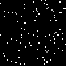
\includegraphics[scale=1]{przyklad.png}
\end{center}
\caption{przykładowe wejście prostej sieci neuronowej}
\label{fig:przyklad_prostego_wejscia}
\end{figure}
\hyperref[fig:przyklad_prostego_wejscia]{Rysunek \ref*{fig:przyklad_prostego_wejscia}} jest rozmiaru 50x50 pikseli i może być przykładem danych wejściowych do sieci neuronowej. Małe zagęszczenie białych pól ułatwia w tym wypadku ich zliczanie. Poprawną odpowiedzią do zadanego przykładu jest 95. 

\subsection{Plan ew. rozbudowy projektu}
\subparagraph{Omówienie} Po zaimplementowaniu i sprawdzeniu działania poprawności wcześniejszego etapu, spróbujemy nieco bardziej rozbudować projekt o niżej opisane punkty.

\subparagraph{Przetwarzanie obrazu}
\begin{enumerate}
\item Przekształcenie obrazu do postaci z pierwszego etapu można wykonać na dwa sposoby. Pierwszym jest użycie obrazu referencyjnego. Uznaje się że nie ma na nim interesujących nas obiektów - na przykład jest to obrazek przedstawiający pustą ulicę. Następnie tworzy się obrazek będący absolutną różnicą dwóch obrazków - referencyjnego i tego na którym chcemy rozpoznać samochody. Można też zastosować rożne filtry, poprawiające uzyskany wynik, jak filtr medianowy. Omówione operacje na obrazach można wykonać za pomocą biblioteki OpenCV.  Przykładowy wynik takiej różnicy przedstawia \hyperref[fig:absdiff]{Rysunek \ref*{fig:absdiff}}.

\begin{figure}[H]
\begin{center}
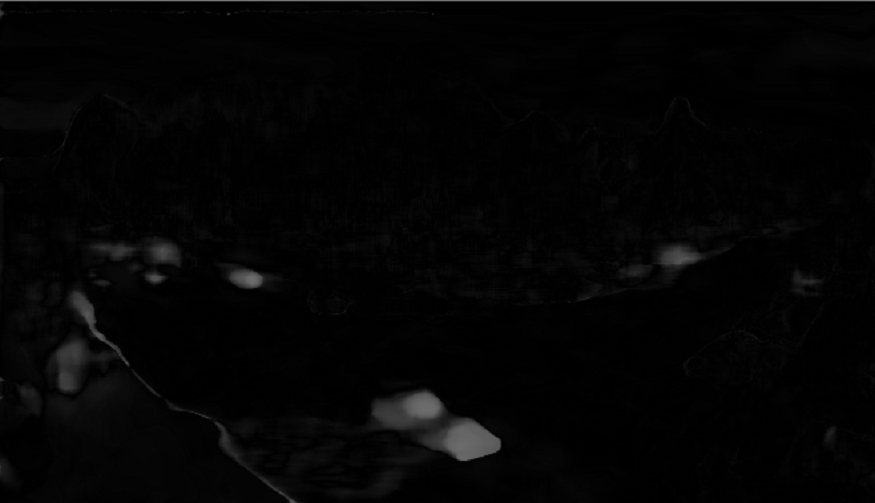
\includegraphics[scale=0.4]{przetwarzanie.png} 
\end{center}
\caption{przykładowy rezultat różnicy obrazów referencyjnego z analizowanym}
\label{fig:absdiff}
\end{figure}

\subparagraph{} Aby znaleźć na takim obrazie konkretne elementy powinno się  usunąć z niego  konsekwencje naturalnych różnic między obrazem referencyjnym a tym na którym chcemy wykryć obiekty, takie jak zmieniające się światło i cień czy zmiany wynikające z podmuchu wiatru. Można skorzystać z funkcji \texttt{threshold}, dzięki której nie tylko pozbędziemy się tych niewielkich różnic ale także uzyskamy obraz na którym są tylko dwa możliwe kolory - czarny lub biały, dzięki czemu kolejne operacje będą łatwiejsze.  Problemem może być dobór odpowiedniej wartości jasności piksela, powyżej której jest on kwalifikowany jako biały, szczególnie, że  czasem samochody mogą mieć inne wartości różnicy w różnych miejscach, co powoduje, że cały samochód może się pojawić jako dwie grupy pikseli . Widać to na wyniku wspomnianej funkcji przedstawionym na \hyperref[fig:threshold]{Rysunku \ref*[fig:threshold]}. Pokazuje on ponadto, że rzeczywiście niewielkie różnice obrazów zostały wyeliminowane, chociaż nadal część z nich pozostało -- np. część wynikająca z przesuwającego się cienia.

\begin{figure}[H]
\begin{center}
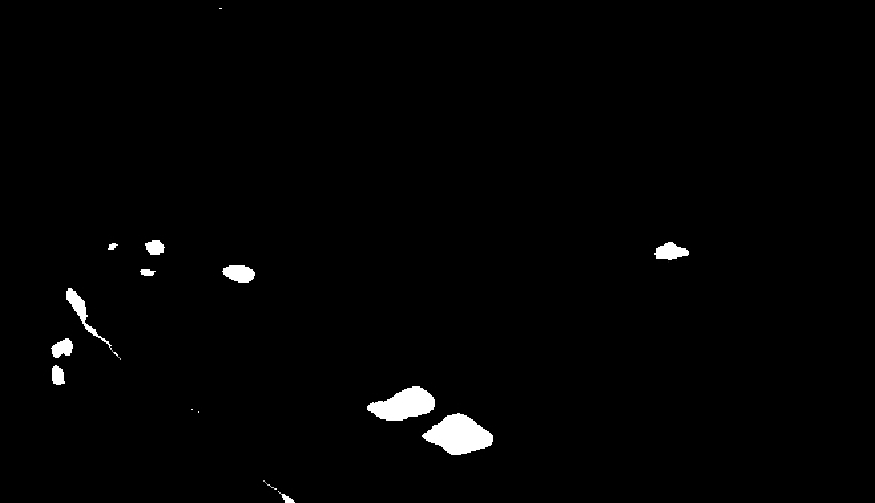
\includegraphics[scale=0.4]{przetwarzanie2.png} 
\end{center}
\caption{\hyperref[fig:absdiff]{Rysunek \ref*{fig:absdiff}} po zastosowaniu funkcji \texttt{threshold}}
\label{fig:threshold}
\end{figure}


\item Drugim sposobem otrzymania obrazu podobnego do poprzedniego jest skorzystanie z klasy BackgroundSubtractor \footnote{\scriptsize \url{http://docs.opencv.org/master/d7/df6/classcv_1_1BackgroundSubtractor.html}}, która sama  na podstawie sekwencji ramek tworzy model tła. Korzysta także z różnicy i funkcji threshold ale wykorzystuje ponadto  mieszaniny gaussowskie - bardziej skomplikowaną metodę.

\begin{figure}[H]
\begin{center}
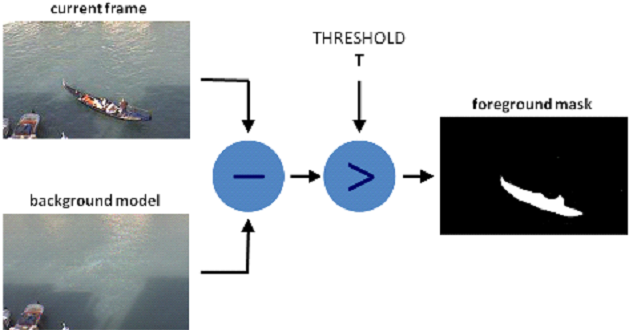
\includegraphics[scale=0.4]{przetwarzanie3.png} 
\end{center}
\caption{To jest background selector, czy schemat działania naszej metody?}
\end{figure}


\item Wykrywanie konturów

\subparagraph{} Wykrywanie konturów pozwala zaklasyfikować zbiór danych pikseli jako jeden fragment. Pomijając kontury o zbyt małym kształcie i nakładające się samochody, które mogą być sklasyfikowane jako jeden kontur, będzie można znaleźć miejsca \quotedblbase podejrzane\textquotedblright o bycie samochodem na zadanym obrazku. Dzięki temu sieć neuronowa zostanie odciążona przez mniejszą ilość danych wejściowych, które mogłyby być kłopotem przy metodzie sliding window i przetwarzaniu całego obrazu od początku.

\begin{figure}[H]
\begin{center}
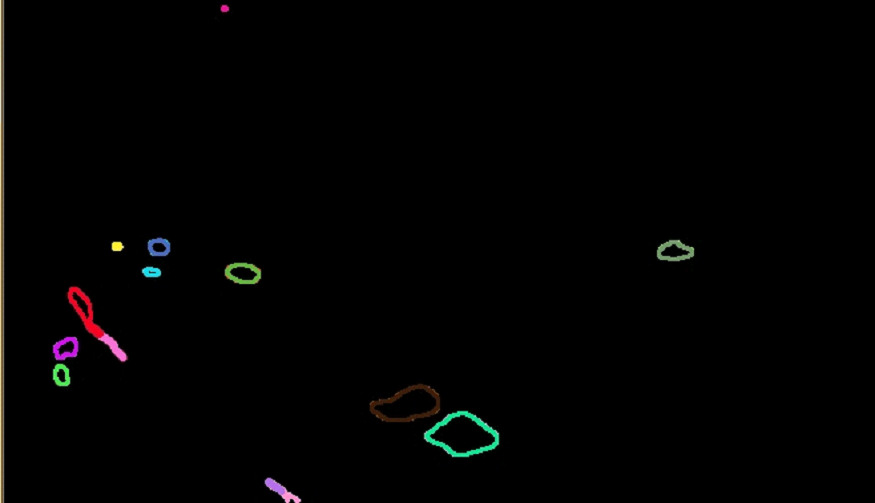
\includegraphics[scale=0.4]{kontury.png} 
\end{center}
\caption{przykład wykrytych konturów}
\label{fig:contours}
\end{figure}

\end{enumerate}

\subparagraph{Rozbudowanie sieci neuronowej} Istnieje możliwość rozbudowania sieci neuronowej o inny typ – SOM ( Self-organising map), która pozwala na rozpoznawanie podobnych obrazków. Wynikiem działania sieci jest klasyfikacja przestrzeni w sposób grupujący zarówno przypadki ze zbioru uczącego, jak i wszystkie inne wprowadzenia po procesie uczenia.  Może to również usprawnić pracę działania programu.

\section{Problemy implementacyjne}
\subsection{Wybór języka programowania}
\subparagraph{} Biorąc pod uwagę dostępność dedykowanych bibliotek oraz ogółem materiałów związanych z tematem naszej pracy, zdecydowaliśmy się na wybór języka C++ \footnote{natywny język OpenCV, FANN, natywny język dla API OpenCL-a}. Dostępność gotowych rozwiązań z jednej strony ułatwia implementację, z drugiej dodatkowo gwarantuje rozsądną szybkość działania, zagwarantowaną przez długotrwałe testowanie opragramowania, jak również sam wybór dosyć nieskopoziomowego języka, jakim jest C++. Dodatkowym argumentem przemawiającym za takim wyborem jest fakt, że każdy z uczestników projektu ma doświadczenie z tym językiem.

\subsection{Biblioteki}
\begin{itemize}
\item \textbf{OpenCV}
\subparagraph{} Jest to biblioteka funkcji wykorzystywanych do przetwarzania obrazów. W naszym projekcie wykorzystujemy funkcje wykonujące operacje takie jak usuwanie szumów, progowanie obrazu, wykrywanie krawędzi.

\item \textbf{OpenCL}
\subparagraph{} Jest to framework wspomagający pisanie programów równoległych, działających na platformach składających się z różnego rodzaju jednostek obliczeniowych (CPU, GPU). Umożliwi on szybsze wykonywanie programu.

\item \textbf{Qt}
\subparagraph{} Aby ułatwić obsługę programu, zdecydowaliśmy się na użycie biblioteki graficznej.  Qt jest biblioteką programistyczną, służąca do budowy graficznego interfejsu programu. Jest biblioteką dedykowaną m.in. dla języka C++. 

\end{itemize}

\subsection{Sieć neuronowa}
\subparagraph{Wybór sieci neuronowej} Podstawową strukturą sieci neuronowej wykorzystywanej w naszym programie jest wielowartstwowy FFANN (ang. Feedforward Artifical Neural Network), pobierająca jako wejście ciąg pikseli podany w kolejności praw- lewo, góra-dół; każdy piksel reprezentowany jest jest przez 32-bitową liczbę w formacie RGBA (8 bitów na kanał).
W czasie wyboru algorytmu uczącego interesowały nas wyniki różnych metod dla zagadnienia wykrywania schematów wśród danych wejściowych. Korzystając z zestawienia porównującego popularne algorytmy uczące \footnote{\scriptsize \url{http://www.mathworks.com/help/nnet/ug/choose-a-multilayer-neural-network-training-function.html}} wybór padł na metodę z rodziny resilient backpropagation. Mając na uwadze prędkość uczenia i prostotę implementacji ostatecznie wybraliśmy algorytm iRPROP+.

\subparagraph{} Razem z wyborem funkcji uczącej, będącej pochodną metody backpropagation, pojawia się problem wyboru funkcji aktywującej dla pojedyńczych neuronów. Jak każdy algorytm tego typu, w celu uaktualnienia wag poszczególnych połączeń między neuronami w sieci, iPROP+ wymaga liczenia pochodnej funkcji błędu względem poszczególnej wagi, która z kolei wymaga znajomości pochodnej funkcji aktywacji. W celu uproszczenia obliczeń przyjęliśmy więc za nią funkcję logicznę postaci ...., której pochodna ma bardzo wdzięczną cechę .... Dzięki temu faktowi poprzednie równanie upraszcza się do dużo łatwiejszej do implementacji postaci:. 

\subparagraph{} Istotnym dla nas założeniem jest, aby implementacje wybranej metody umożliwiała dynamiczne dostowanie wielkości wiejścia i ilości warstw, dzięki czemu możliwe będzie stworzenie kilku niezależnych sieci, wykorzystwywanych dla wycinków analizowanej klatki o różnych rozmiarach. Zakładając, że fragment podejrzany o zawieranie samochodu ma wymiary 50x50, a my dysponujemy sieciami przyjmującymi 60x60 i 30x30, określenie całośćiowego prawdopodobieństwa dla podanego wejścia może być policzone jako ważona suma wyjść każdej sieci, gdzie wagą jest bliskość oryginalnego rozmiaru wejścia w stosunku do faktycznego wejścia danej sieci. Takie podejście upodabnia całość rozwiązania do opisanej na początku metody Multinet, gdzie na obliczenie ostatecznego rezultatu skłądały się wyniki wielu sieci.

\subparagraph{Problem zrównoleglenia} Wybrany przez nas typ sieci ma tę zaletę, że dosyć łatwo daje się zrównoleglić. Korzystamy tutaj z faktu, że w czasie liczenia wyniku całej sieci, jeśli poprzednia warstwa zakończyła już liczenie wyjść swoich neuronów, dane będące na wejściu kolejnej są dobrze określone i nie podlegają zmianom w czasie liczenia wyjścia następnej warstwy. Jedyne konflikty w dostępnie do pamięci, w obrębie jednej wartwy, mogą mieć miejsce w chwili wyliczania $x$ dla funkcji aktywacji $i$-tego nauronu w danej wartstwie. Zakładając istnienie $m$ przychodzących połączeń, \[x_i = \sum _{j=0}^{m}w_{i,j}*in_j\]. Mamy więc $m$ konkurujących ze sobą wątków, chcących jednocześnie modyfikować tę samą zmienną $x_i$. Z pomocą przychodzą nam tutaj operaje atomowe, obsługiwane przez OpenCL. Ogólnie, przy zastosowaniu odpowiedniej liczby wątków, jesteśmy w stanie zrównoleglić działanie sieci typu Feedforward w taki sposób, aby każda operacja wymagała $O(n)$ kroków, gdzie $n$ jest liczbą warstw.


\newpage
\listoffigures

\end{document}